\documentclass{article}
\usepackage{blindtext}
\usepackage[a4paper, total={6in, 9.4in}]{geometry}
\usepackage{indentfirst}
\usepackage{wrapfig}
\usepackage{graphicx}
\usepackage{mathtext}
\usepackage{amsmath}
\usepackage{siunitx} % Required for alignment
\usepackage{subfigure}
\usepackage{multirow}
\usepackage{rotating}
\usepackage{afterpage}
\usepackage[T1,T2A]{fontenc}
\usepackage[russian]{babel}
\usepackage{caption}
\usepackage[arrowdel]{physics}
\usepackage{booktabs}

\graphicspath{{pictures/}}

\title{\begin{center}Лабораторная работа №4.5.3\end{center}
Сканирующий интерферометр}
\author{Гёлецян А.Г.}
\date{\today}

\begin{document}

\pagenumbering{gobble}
\maketitle
\newpage
\pagenumbering{arabic}

\textbf{Цель работы:} Знакомство с устройством и работой газового лазера
непрерывного действия, со спектральными характеристиками лазер-
ного излучения, а также с устройством и принципом действия скани-
рующего интерферометра Фабри—Перо.

\section{Теоретическая часть}
\subsection{Спектр лазера}
В He–Ne-лазерах используются резонаторы, фактически представляющие собой интерферометр
Фабри—Перо. Излучение распространяется вдоль оси интерферометра. При этом генерируются
моды (типы колебаний), для которых на длине резонатора укладывается целое число полуволн
($L$ -- база интерферометра):

\begin{equation}
    2L=m\lambda
    \label{eq:mode_distance_lambda}
\end{equation}

Из этой формулы получаем разность частот соседних мод

\begin{equation}
    \nu_{m+1} - \nu_{m} = \frac{c}{2L}
    \label{eq:mode_distance_freq}
\end{equation}

Для интерферометра с базой L = 0,6 м межмодовое расстояние равно
250 МГц. В то же время спектральная линия рабочего перехода неона
имеет ширину порядка 1500 МГц, поэтому возможна одновременная
генерация нескольких мод. Рис. \ref{fig:multimodes} иллюстрирует увеличение числа мод
генерации лазера с ростом усиления активной среды.

\begin{figure}[h]
    \center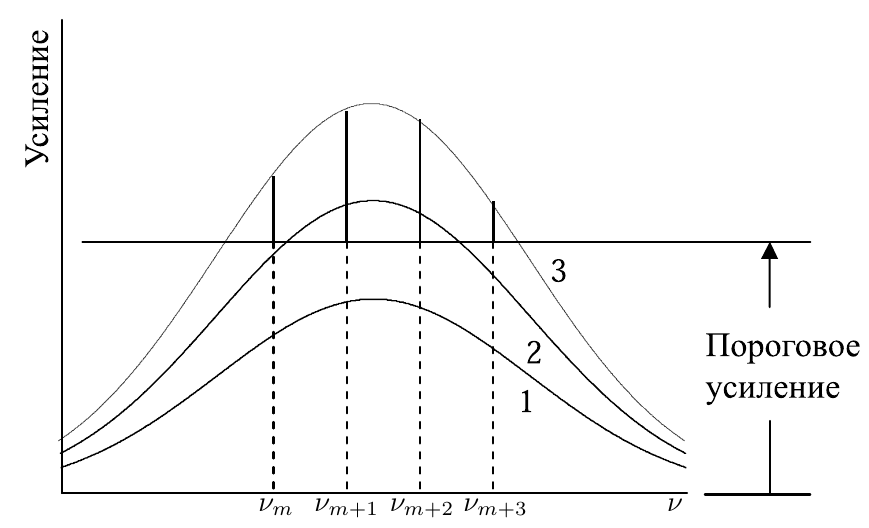
\includegraphics[width = 0.6\linewidth]{multimodes.png}
    \caption{Увеличение числа генерирующих мод при увеличении усиления}\label{fig:multimodes}
\end{figure}

При небольшом усилении (кривая 1) генерации нет. В случае 2 генерация происходит
только на 2 частотах $\nu_{m+1}$ и $\nu_{m+2}$ , расположенных вблизи центра
спектральной линии. Если усиление определяется кривой 3, генерация возникает на
четырёх частотах от $\nu_m$ до $\nu_{m+3}$. Говорят, что в этом случае лазер
одновременно работает на четырёх модах.

Для гелий-неонового лазера с достаточно длинной трубкой на переходе 632.8 нм
многомодовая генерация является обычным режимом работы.

\subsection{Сканирующий интерферометр}
Для исследования межмодового состава излучения He–Ne-лазера в работе используется
сканирующий интерферометр, представляющий собой высокодобротный интерферометр
Фабри–Перо с периодически изменяемой базой. Его устройство схематически показано
на рис. \ref{fig:interferometr}.
\newpage

\begin{figure}[h]
    \center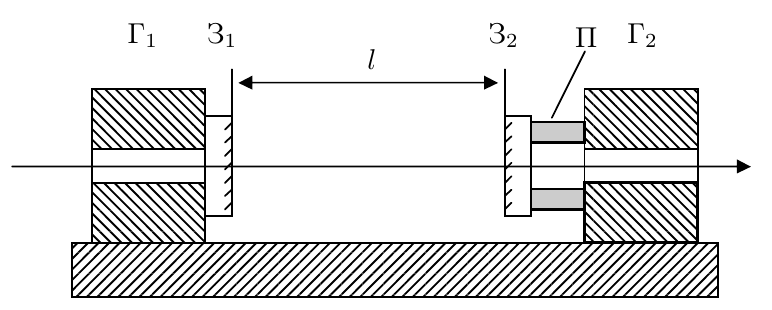
\includegraphics[width = 0.6\linewidth]{interferometr.png}
    \caption{Устройство сканирующего интерферометра}\label{fig:interferometr}
\end{figure}

Если вдоль оси интерферометра распространяется световое излучение с длиной
волны $\lambda$, то при выполнении условия

\begin{equation}
    2l=m\lambda
    \label{eq:fabri_resonanse}
\end{equation}
возникает резонанс, и внешнее излучение полностью проходит через интерферометр.
Собственные моды интерферометра отличаеются по частоте на величину
\begin{equation}
    \Delta \nu = \frac{c}{2l}
    \label{eq:mode_distance_freq_fabri}
\end{equation}
или в единицах $\lambda$
\begin{equation}
    \Delta \lambda_{си} = \frac{\lambda}{m} = \frac{\lambda^2}{2l}
    \label{eq:mode_distance_lambda_fabri}
\end{equation}

Пьезокерамический элемент П периодически изменяет длину интерферометра на величину
порядка $\lambda$, благодаря чему ``плавает'' $l$, и, соответственно, частота сканирования
интерферометра. Если амплитуда колебания зеркала небольшая ($\leq \lambda/2$), то
размытые спектральные пики не перекрываются, и мы получаем одинарную развертку. При
больших амплитудах развертка клонируется (начинается сканирование следующей модой
интерферометра), и получается многократная развертка спектра
(см. рис. \ref{fig:clone_spectrum})

\begin{figure}[h]
    \center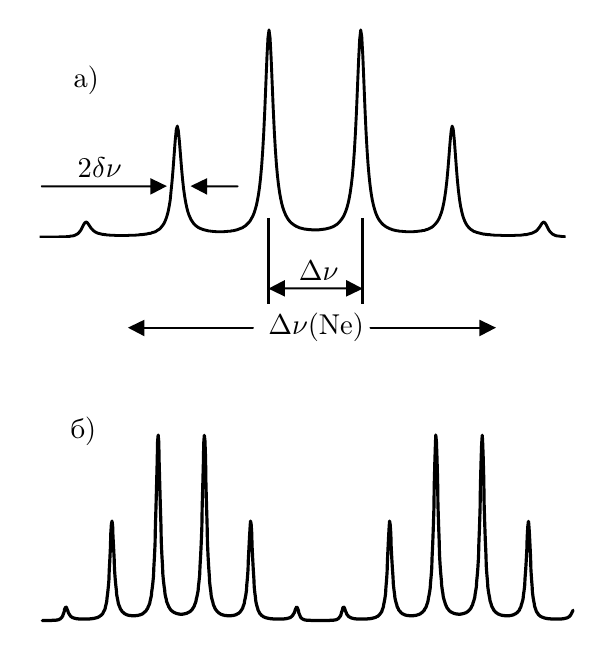
\includegraphics[width = 0.6\linewidth]{clone_spectrum.png}
    \caption{Раздвоение развертки при большрй амплитуде колебания зеркала}\label{fig:clone_spectrum}
\end{figure}

\newpage
\subsection{Экспериментальная установка}
\begin{figure}[h]
    \center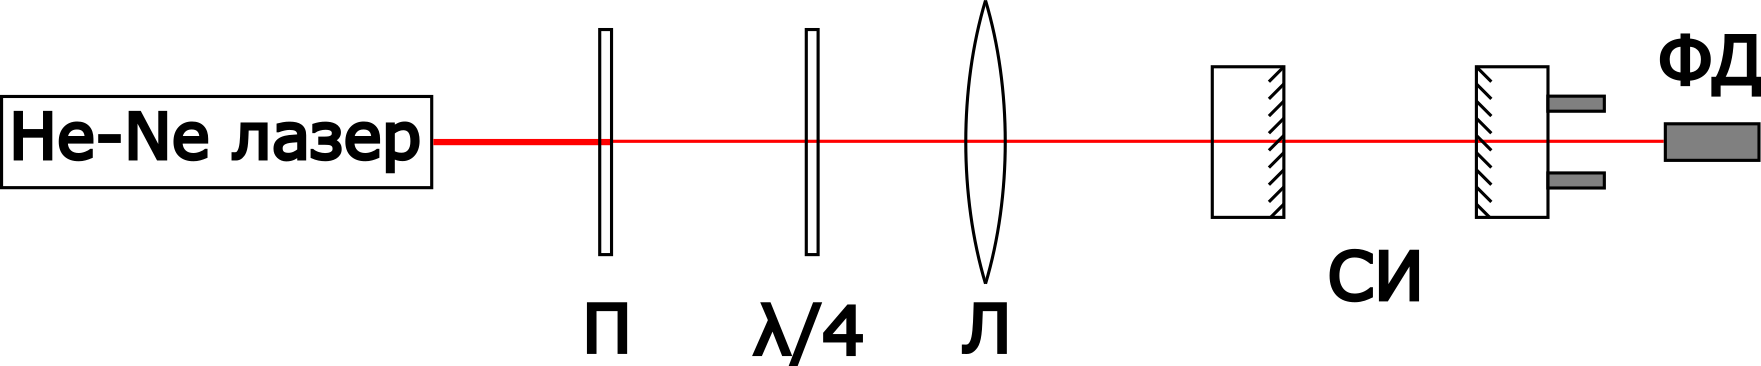
\includegraphics[width=0.9\linewidth]{ustanovka.png}
    \caption{Схема установки}\label{fig:ustanovka}
\end{figure}

Луч лазера проходит через поляризационную развязку, состоящую из поляроида и пластинки
$\lambda/4$. Главное направление пластинки $\lambda/4$ повернуто на $45^\circ$
относительно главного направления поляроида, вследствии чего луч на выходе приобретает
циркулярную поляризацию. При отражении от линзы или зеркал, круговая поляризация
меняет направление, и после прохождения через пластинку $\lambda/4$ приобретает
линейную поляризацию, перпендикулярную разрешенному направлению поляроида. Таким
путем ограничивается световой поток обратно в лазер, благодаря чему добивается лучшее
усиление в трубке лазера.

Линза уменьшает расхождения пучка, поступающего на вход интерферометра. Амплитуда
колебания заднего зеркала регулируется через блок питания, а сигнал с фотодиода
разворачивается на осциллографе, давая спектр излучения.
 
\section{Ход работы}
Параметры установки

\begin{align*}
    \text{База интерферометра: \ \ } l&=9\text{ см}\\
    \text{База лазера: \ \ } L&=65\text{ см}\\
    \text{Длина волны излучения: \ \ } \lambda&=6238 \text{ \AA}
\end{align*}

Центрируем установку, настраиваем поляризационную развязку.

\begin{figure}[h]
    \center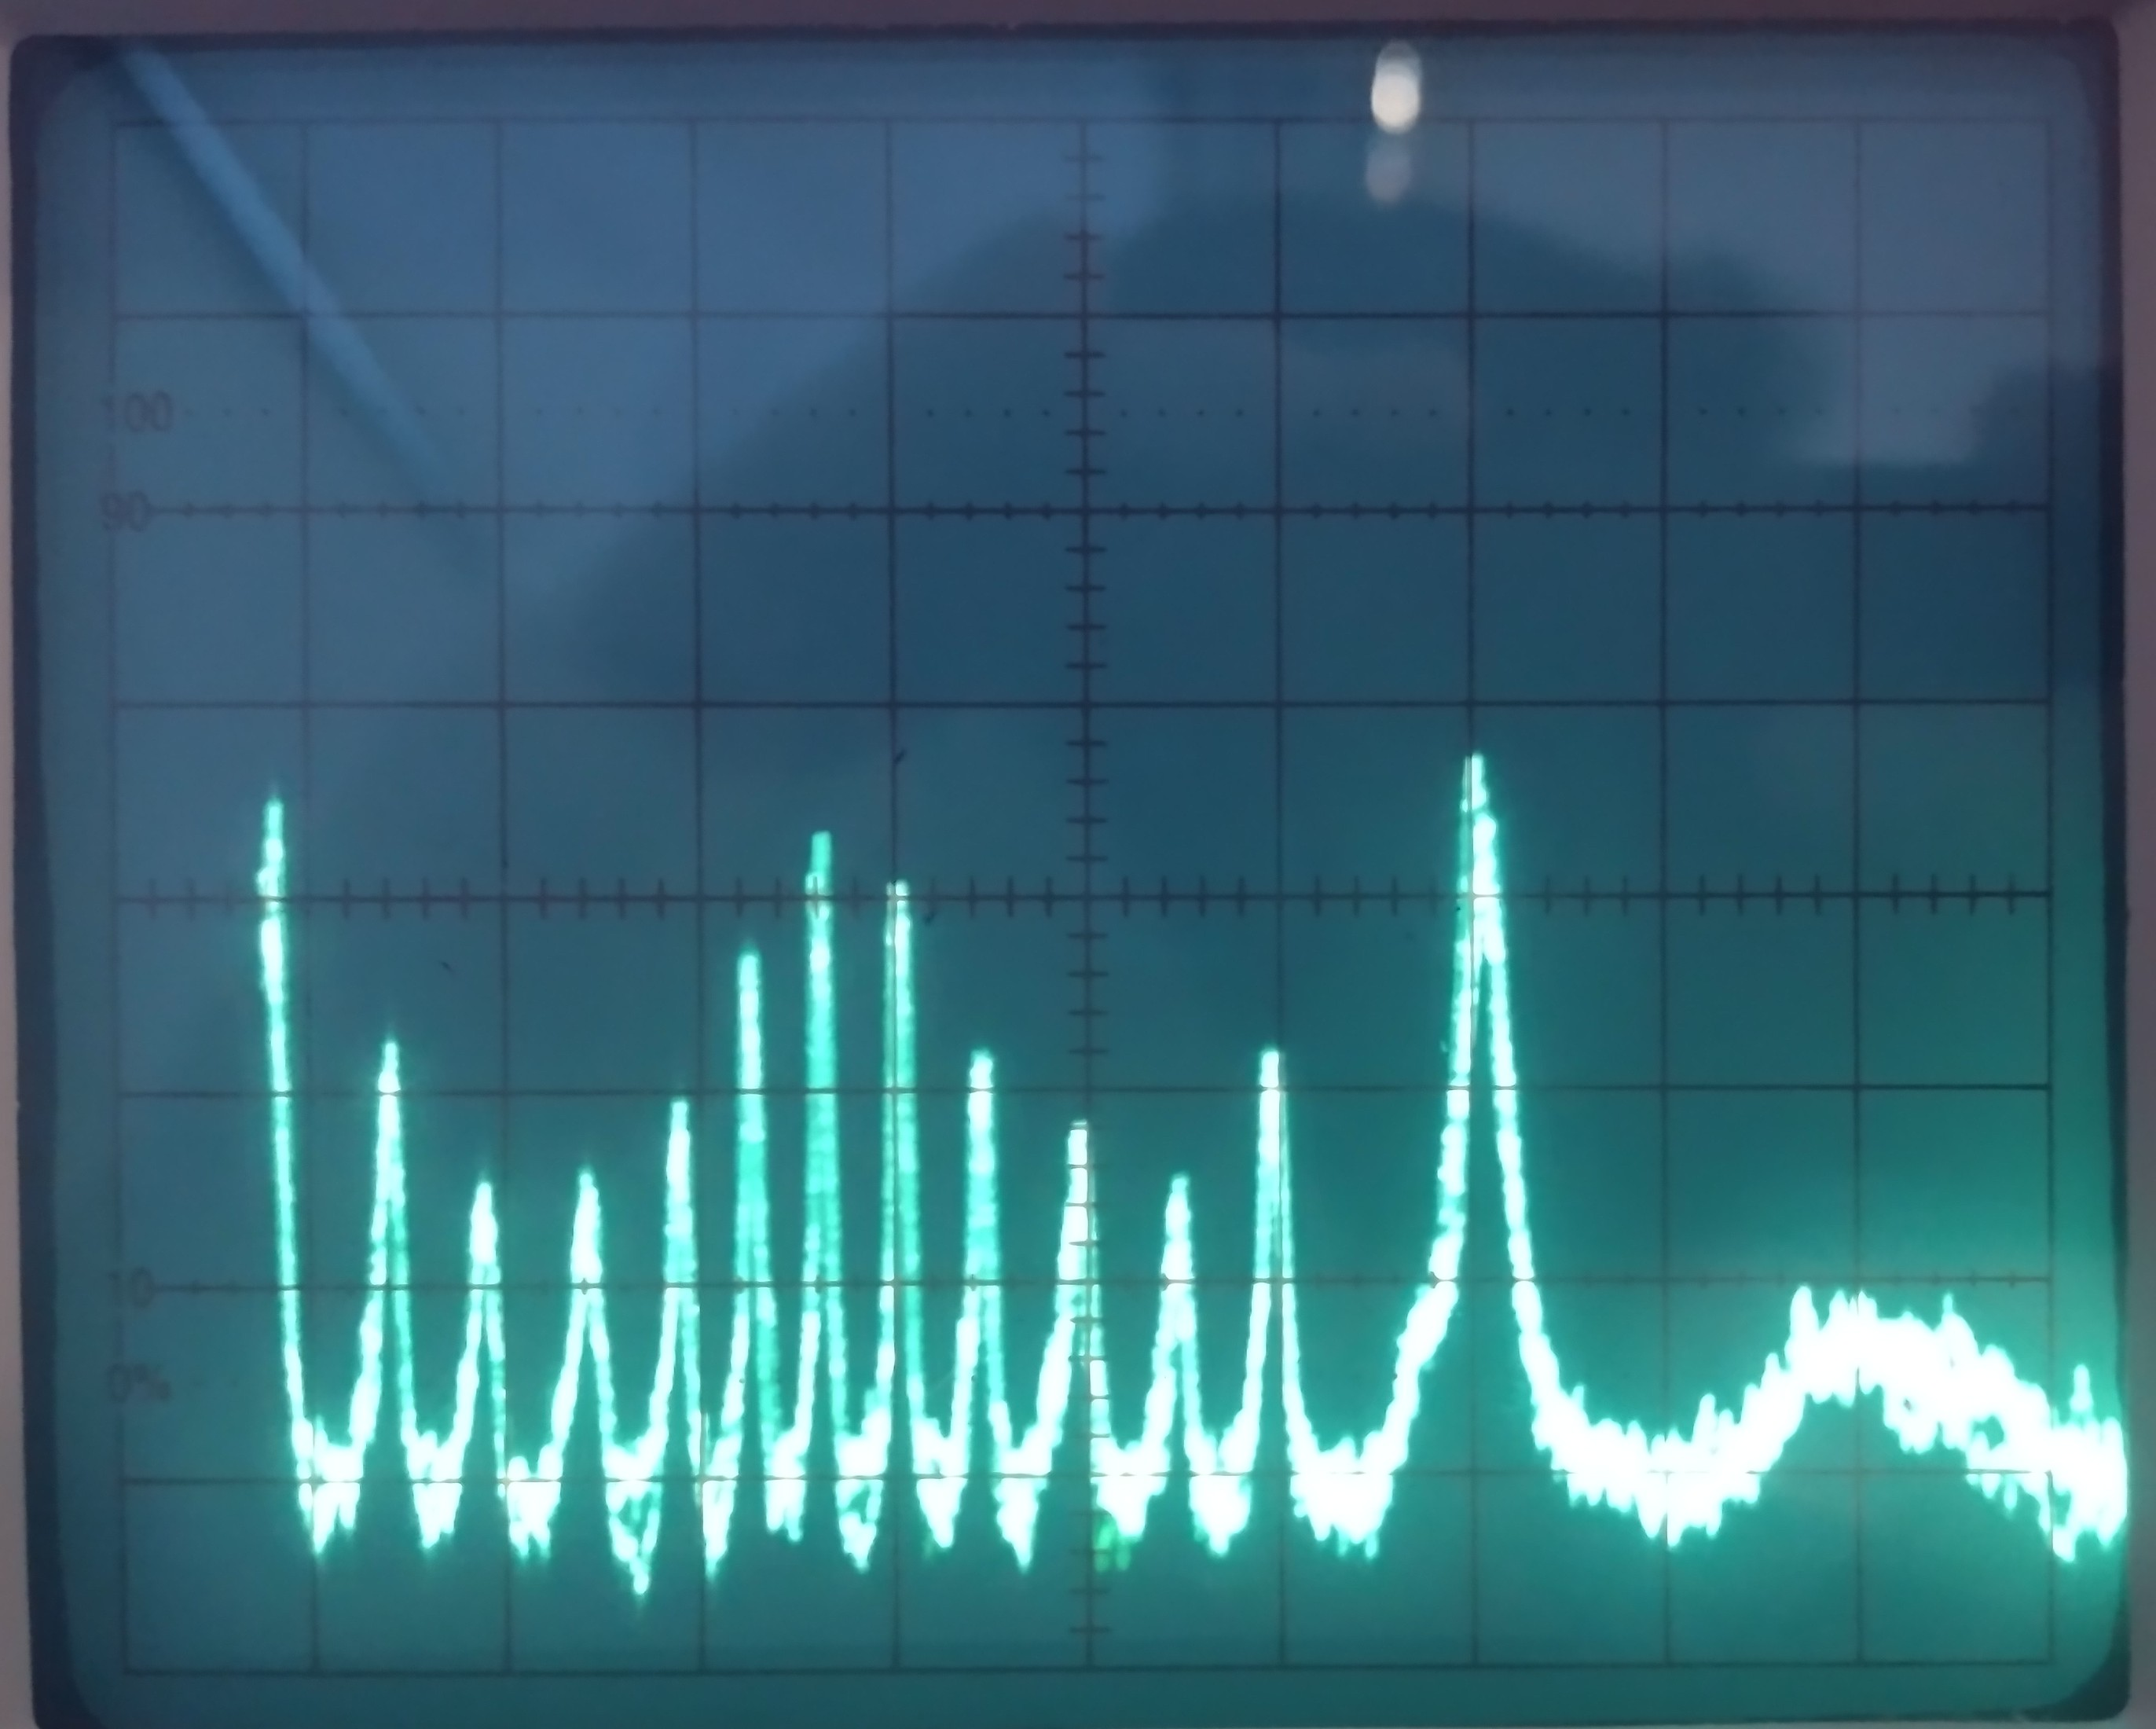
\includegraphics[width=0.5\linewidth]{spectrum_1.jpg}
    \caption{Развертка спектра лазера}\label{fig:spectrum_1}
\end{figure}

На рис.~\ref{fig:spectrum_1} виден удвоенный спектр гауссовского профиля
излучения лазера. В одном профиле помещается $N=7$ мод. Полуширина профиля
\begin{equation}
    \Delta\lambda(\text{Ne})=\frac{N}{2} \frac{\lambda^2}{2L} \approx
    10.8 \cdot 10^{-3}\text{ \AA}
\end{equation}

Предполагая, что ширина спектральной линии обусловлена эффектом Доплера, можем оценить
температуру лазерной трубки.

\begin{equation}
    \frac{\Delta\lambda(\text{Ne})}{\lambda}\approx\frac{v_x}{c}
    \text{;\ \ \ } \frac{m{v_x}^2}{2} \approx \frac{kT}{2}
\end{equation}
В данной модели получаем температуру трубки $T\approx 637$ К.

\paragraph{}
Дисперсионная область интерферометра, рассчитанная по
формуле (\ref{eq:mode_distance_lambda_fabri}): $\Delta\lambda_{си} \approx 22.2\cdot10^3$
\AA\@. 

\paragraph{}
Оценим разрешающую способность интерферометра, измеряя ширину моды на полувысоте.

\begin{figure}[h]
    \center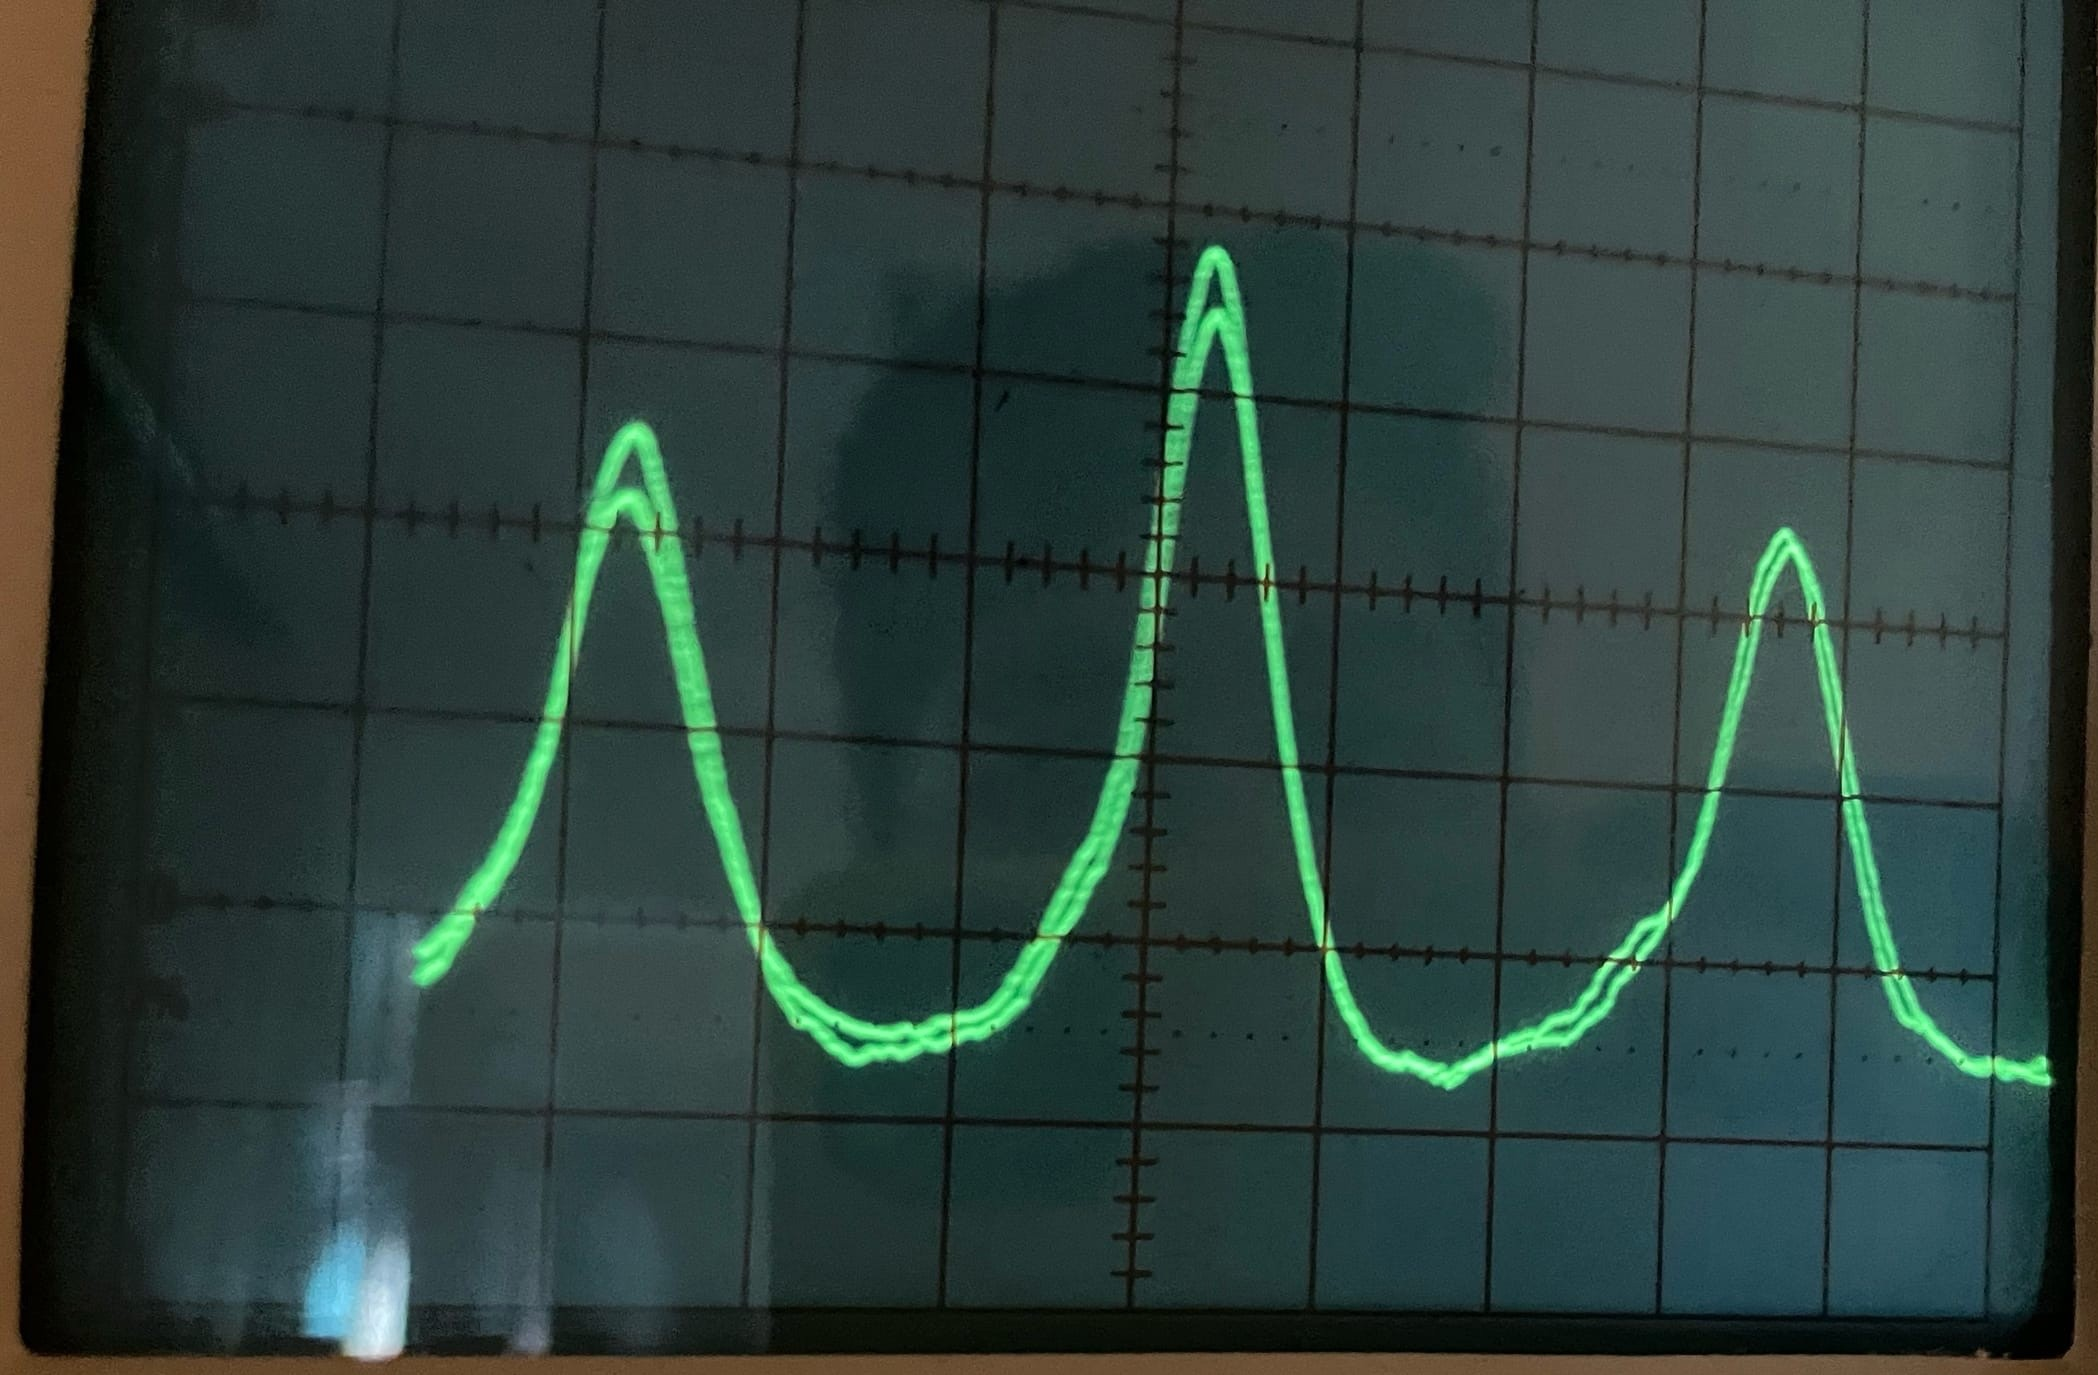
\includegraphics[width=0.5\linewidth]{solo_peak.jpg}
    \caption{Спектр трех мод лазера}\label{fig:solo_peak}
\end{figure}

Расстояние между пиками $3.4$ клеток, что соответствует
$\Delta\lambda = 3.08\cdot10^{-3}$ \AA\@. Ширина на полувысоте состовляет $0.8$ клеток,
что соответствует $\delta\lambda = 0.72 \cdot 10^{-3}$ \AA\@. Разрешающая способность
$R=\lambda/\delta\lambda\approx8.8\cdot10^6$.

Разрешающая способность интерферометра Фабри-Перо
\begin{equation}
    R = \frac{2\pi l}{\lambda(1-r)}
\end{equation}
Отсюда можем оценить коэффициент отражения зеркал: $r\approx0.90$

\section{Выводы}
В ходе работы получили температуру лазерной трубки примерно $370^\circ$ C, что
не соответствует действительности, судя по ощущениям руки, а так же исходя из той логики,
что блок питания не имеет достаточной мощности для поддержания данной температуры.

Так же стоит заметить, что $2\Delta \lambda\text{(Ne)}$ подозрительно близко похож
на $\Delta \lambda_{си}$, что может означать неполное исследование спектра лазера
(полоса пропускания интерферометра обрезает спектр лазера).

В целом, на качественном уровне наблюдения удачные, но установка не приспособлена
для количественных измерений.

\end{document}

